\documentclass[../report.tex]{subfiles}
\graphicspath{{\subfix{../image/}}}

\begin{document}
\maketitle

\subsection{Versions \& Assembly System}
Implementation of  the versioning into the CAD-design allowed us to have a clear overview
of the current state of the project, while still being able to come back and compare to older 
versions. 
A version only updates after the part has been produced. All changes before 
printing or manufacturing are part of that version.

The assembly system is a combination of the assembly application of the CAD-Software
in addition with a folder structure that shows clearly where parts of certain categories 
are supposed to be saved. Now a new part can be created within the specific subassembly and 
saved in the subassembly folder or a existing part can be added to the specific folder and 
then implemented into the subassembly. 

This prevents file clustering or having one confusing folder containing all files and one opening 
and reopening of different versions can look like this, with the final version on the right:
\begin{figure}[H]
    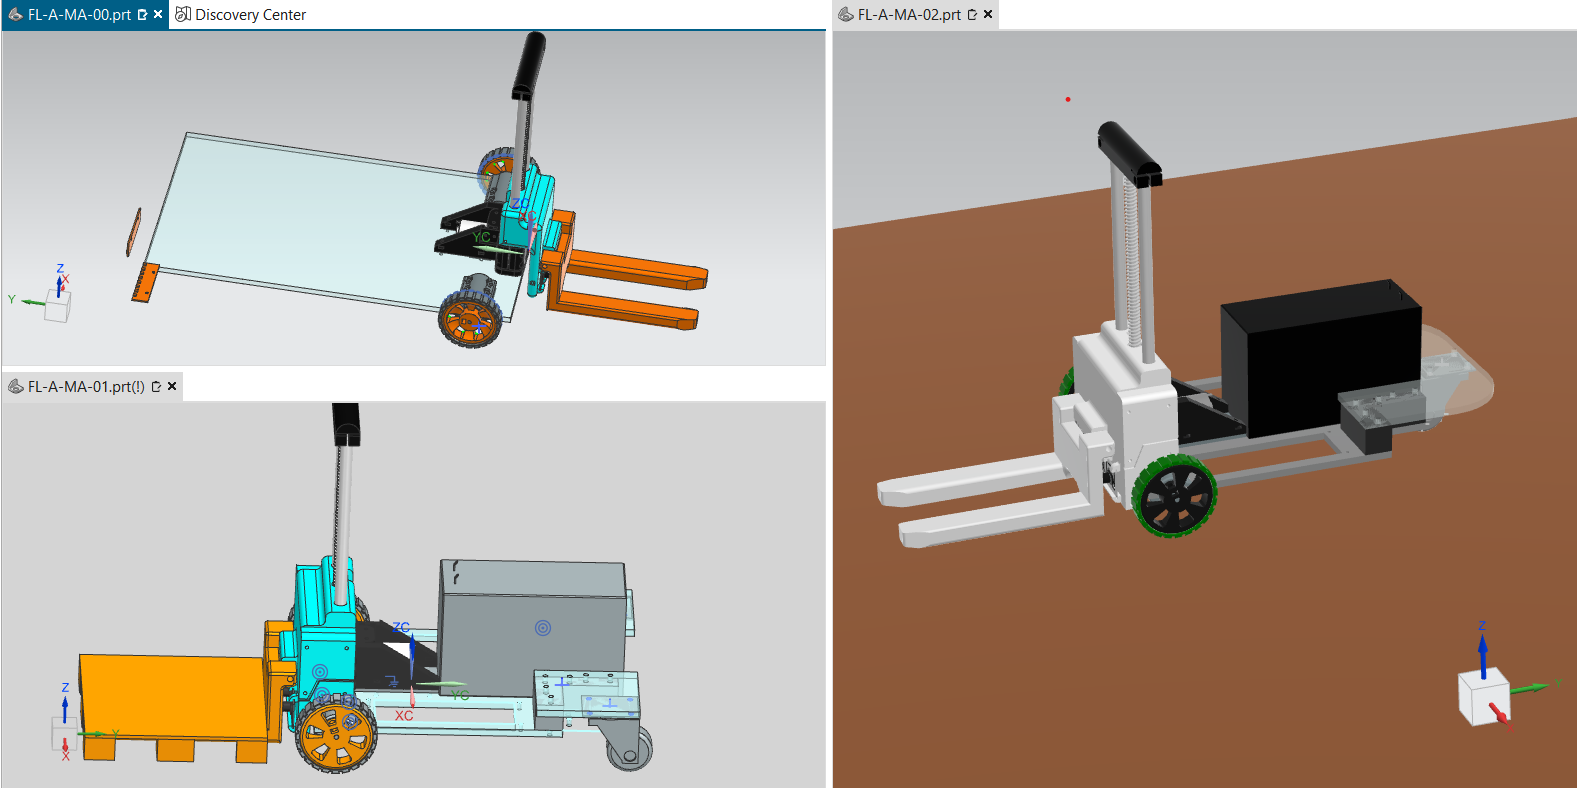
\includegraphics[width=\textwidth]{all.png}
\end{figure}



\end{document}